% Let $\mathcal{C}$ be an arbitrary category. 
% The type graph method is parameterized by a tuple \(\mathcal{T} = (T, \mathbb{E}, \mathcal{S}, w)\), called a \textbf{weighted type graph}~\cite{endrullis2024generalized_arxiv_v2}, consists of:
%     \begin{itemize} 
%         \item an object \(T\) in $\mathcal{C}$, called \textbf{type graph},
%         \item a strongly monotonic, measurable semiring \(\mathcal{S}=(S, \oplus, \odot, 0_\mathcal{S}, 1_\mathcal{S}, \prec, \mu)\),
%         \item a set \(\mathbb{E}\) of morphisms with codomain $T$ in $\mathcal{C}$, called \textbf{morphism-rulers}, 
%         \item a weight function \(w : \mathbb{E} \to S \setminus \{0_\mathcal{S}\}\),
%         \item for every \( (e :X \to T) \in \mathbb{E}\) and every object \(G\), the sets \(\operatorname{Hom}(X, G)\) and \(\operatorname{Hom}(G, T)\) are finite.
%     \end{itemize}

% \begin{example}
%     \label{example:weighted_type_graph}
%      In \textbf{Graph}, a weighted type graph can be visualized as a graph with weighted labels and weights given as superscripts as proposed in \cite{bruggink2015proving} if $\operatorname{dom}(\mathbb{E})$ consists of graphs with two vertices and one labeled edge between them. For example, the weighted type graph $\mathcal{T} = (T, \mathbb{E}, \mathcal{S}, w)$ with $\mathcal{S}$ as the real arithmetic semiring $(\mathbb{R}^+, +, *, 0_\mathbb{R}, 1_\mathbb{R}, <, \operatorname{id}_{\mathbb{R}^+})$,
%      $T$ as the graph illustrated below (without superscripts), $\mathbb{E}=\{e_{11a},e_{12a},e_{21a},e_{11b}\}$ as the set of morphism-rulers where 
%      $e_{uvl}$ has domain 
%      \tikz[baseline=-0.5ex]{
%         \node (x) at (0,0) {$\bullet$};
%         \node (y) at (1,0) {$\bullet$};
%         \draw[->] (x) -- (y) node[midway, above] {$l$};
%     } and image 
%     \begin{tikzpicture}
%         \node[draw, circle] (x) at (0,0) {$\mathrm{u}$};
%         \node[draw, circle] (y) at (1,0) {$\mathrm{v}$};
%         \draw[->]  (x) -- (y) node [midway,above] {$l$};
%     \end{tikzpicture} in the graph $T$,
%     and $w(e) = 1$ for all $e \in \mathbb{E}$, can be visualized as follows:
%     \begin{center}
%         \begin{tikzpicture}
%             \graphbox{}{0mm}{0mm}{32mm}{28mm}{-10mm}{-14mm}{
%                 \node[draw,circle] (1) at (0,0) {1};
%                 \node[draw,circle] (2) at (2,0) {2};
%                 \draw[->] (1) edge[loop above] node[midway, above] {$a^{1}$} (1) ;
%                 \draw[->] (1) edge[loop below] node[midway, below] {$b^{1}$} (1) ;
%                 \draw[->] (1) edge[bend left] node[midway, above] {$a^{1}$}  (2)  ;
%                 \draw[->] (2) edge[bend left] node[midway, below] {$a^{1}$} (1)   ;
%             }
%         \end{tikzpicture}
%     \end{center}
% \end{example}

% Let \(\mathcal{T} = (T, \mathbb{E}, \mathcal{S}, w)\) be a weighted type graph and \(G\) an object of the category $\mathcal{C}$.

% Analogous to measuring a physical object, a morphism ruler measures a morphism.
% Let \(\mathcal{T} = (T, \mathbb{E}, \mathcal{S}, w)\) be a weighted type graph and \(G\) an object of the category $\mathcal{C}$. Consider the morphism-ruler \(e\colon X\to T\) and the morphism \(h\colon G\to T\) in~\ref{fig:wf:measurement_of_a_morphism_relative_to_a_morphism_ruler}. The measurement of \(h\) relative to \(e\) is the number of morphisms \(\iota\colon X\to G\) with \(h\circ\iota = e\). 
In this section, we recall the definition of morphism weight and object weight relative to a type graph presented in~\cite{endrullis2024generalized_icgt}.
% Analogous to measuring a physical object, a morphism ruler measures a morphism by counting the maps \(\iota\) that make the triangle in Figure~\ref{fig:wf:measurement_of_a_morphism_relative_to_a_morphism_ruler} commute. Concretely, given a morphism-ruler \(e\colon X\to T\) and a morphism \(h\colon G\to T\), the measurement of \(h\) relative to \(e\) is the number of morphisms \(\iota\colon X\to G\) with \(h\circ\iota = e\).

    % Analogous to the measurement of a physical object, a morphism-ruler measures a morphism, and provides a measurement, which is the number of $\iota$ that make the commutative triangle shown in Figure~\ref{fig:wf:measurement_of_a_morphism_relative_to_a_morphism_ruler}.
\begin{notation}[\cite{endrullis2024generalized_arxiv_v2}]
Let \(A,B,C\) be objects. For morphism $\alpha\colon A\to B$, we introduce the notation 
          $$\set{ \alpha \star - = \gamma } \overset{\operatorname{def}}{=} \{ \beta \in \operatorname{Hom}(B, C) \mid \alpha \star \beta = \gamma \}$$ 
For morphism $\beta\colon B\to C$, we introduce the notation
          $$\set{ - \star \beta = \gamma }  \overset{\operatorname{def}}{=} \{ \alpha \in \operatorname{Hom}(A, B) \mid \alpha \star \beta = \gamma \}$$
For morphism set $E \subseteq \operatorname{Hom}(A,B)$ and morphism $\beta\colon B\to C$, we introduce the notation
          $$E \star \beta \overset{\operatorname{def}}{=} \set{ \alpha \star \beta \mid \alpha \in E }$$
\end{notation}
Analogous to measuring a physical object, a morphism ruler measures a morphism (Definition~\ref{def:measurement_of_a_morphism_relative_to_a_morphism_ruler}).
Let \(\mathcal{T}=(T,\mathbb{E},\mathcal{S},w)\) be a weighted type graph and let \(G\) be an object of the category \(\mathcal{C}\).
Given a morphism-ruler \(e\colon X\to T\) and a morphism \(h\colon G\to T\) as shown below:
\begin{center}
        % \centering
            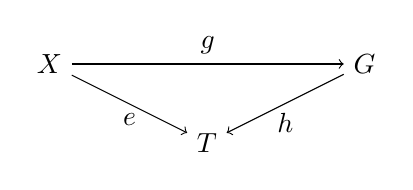
\begin{tikzpicture}
                \node (a) at (0,0) {$X$};
                \node (c) at (4,0) {$G$};
                \node (d) at (2,-1) {$T$};
                \draw[->] (a) -- (d) node [midway,below] {$e$};
                \draw[->] (a) -- (c) node [midway,above] {$g$};
                \draw[->] (c) -- (d) node[midway, below] {$h$};
                % \node (d) at (2,-0.5) {=};
            \end{tikzpicture}
        % \caption{}
        % \label{fig:wf:measurement_of_a_morphism_relative_to_a_morphism_ruler}
    \end{center}  
% in Figure~\ref{fig:wf:measurement_of_a_morphism_relative_to_a_morphism_ruler},
The measurement of \(h\) relative to \(e\) is the number of morphisms \(g \colon X\to G\) with \(h\circ g = e\). 
\begin{definition} 
    \label{def:measurement_of_a_morphism_relative_to_a_morphism_ruler}
    The \emph{measurement} of a morphism \( h:G \to T \) relative to a morphism-ruler \( e: X \to T \), denoted by $m_e(h)$, is defined as:
                \(
                m_e(h) 
                    \overset{\operatorname{def}}{=}
                \card{\{- \star h = e\}}
                \)
\end{definition}
Combining the measurements of a morphism provided by all morphism-rulers with the help of a weight function $w$ gives the weight of the morphism (Definition~\ref{def:weight_of_a_morphism_relative_to_a_type_graph}).
 We define the exponentiation operation for elements of the semiring before defining formally the morphism weight.
\begin{notation} 
    \label{wfs:def:exponentiation}
Let $(S, \oplus, \odot, 0_S, 1_S)$ be a semiring. We define the \textbf{exponentiation operation} for all $x \in S$ and $n \in \mathbb{N}$ by
   \begin{itemize}
        \item $ x^0 \isdef 1_S$,
        \item $x^{n+1} \isdef x^n \odot x$
   \end{itemize}
\end{notation}
\begin{definition} 
    \label{def:weight_of_a_morphism_relative_to_a_type_graph}
        Let $\mathcal{T}=(T,\mathbb{E},\mathcal{S},w)$ be a finitary weighted type graph.
         The \textbf{weight of a morphism $h: G \rightarrow T$ relative to a type graph $\mathcal{T}$} is defined as the semiring product of $w(e)^{m_e(h)}$ for all $e \in \mathbb{E}$:
        \[  w_{\mathcal{T}}(h) \overset{\operatorname{def}}{=} \underset{e \in \mathbb{E}}{\bigodot} 
                w(e)^{m_e(h)} \]
\end{definition}
Finally, the weight of an object is defined as the semiring sum of the weights of all morphisms from the object to the underlying type graph $T$ of the weighted type graph $\mathcal{T}$.
\begin{definition}[Object weight]
    \label{def:weight_of_an_object_relative_to_a_type_graph}
       Let $\mathcal{T}=(T,\mathbb{E},\mathcal{S},w)$ be a finitary weighted type graph. The \textbf{weight of an object \( G \)} is defined as the semiring sum of $w_\mathcal{T}(h)$, for all \( h \in \operatorname{Hom}(G,T) \):
        \[ w_\mathcal{T}(G) \overset{\operatorname{def}}{=} \underset{h \in \operatorname{Hom}(G,T)}{\bigoplus}  w_\mathcal{T}(h) \]
\end{definition}

\begin{example}
    Consider the two morphisms shown below
    %  Figure~\ref{fig:example:two_weighted_type_graph_morphisms}
    % \begin{figure}[H]
    %     \centering
    \begin{center}
        \resizebox{0.7\textwidth}{!}{
        \begin{tikzpicture}
          \graphbox{\( L \)}{-50mm}{0mm}{40mm}{39mm}{2mm}{-6mm}{
            \coordinate (o) at (0mm,-10mm); 
            \node[draw,circle] (l1) at ($(o)+(-10mm,0mm)$) {1};
            \node[draw,circle] (l2) at ($(l1)+(2,0)$) {2};
            \node[draw,circle] (l3) at ($(l1) + (1,0)$) {3};
            \draw[] (l1) -- (l3) node[midway,above] {$a$};
            \draw[] (l3) -- (l2) node[midway,above] {$a$};
        } 
            \graphbox{$T$}{0mm}{0mm}{40mm}{39mm}{-10mm}{-17mm}{
                \node[draw,circle] (1) at (0,0) {$1\ 2$};
                \node[draw,circle] (2) at (2,0) {3};
                \draw[->] (1) edge[loop above] node[midway, above] {$a^{1}$} (1) ;
                \draw[->] (1) edge[loop below] node[midway, below] {$b^{1}$} (1) ;
                \draw[->] (1) edge[bend left] node[midway, above] {$a^{1}$}  (2)  ;
                \draw[->] (2) edge[bend left] node[midway, below] {$a^{1}$} (1)   ;
            }
            \node () at (-5mm,-15mm) {$\overset{h_{11}^1}{\to}$};
        \end{tikzpicture}
        }

        \resizebox{0.7\textwidth}{!}{
            \begin{tikzpicture}
              \graphbox{\(L\)}{-50mm}{0mm}{40mm}{39mm}{2mm}{-6mm}{
                \coordinate (o) at (0mm,-10mm); 
                \node[draw,circle] (l1) at ($(o)+(-10mm,0mm)$) {1};
                \node[draw,circle] (l2) at ($(l1)+(2,0)$) {2};
                \node[draw,circle] (l3) at ($(l1) + (1,0)$) {3};
                \draw[] (l1) -- (l3) node[midway,above] {$a$};
                \draw[] (l3) -- (l2) node[midway,above] {$a$};
            } 
                \graphbox{$T$}{0mm}{0mm}{40mm}{39mm}{-10mm}{-19mm}{
                    \node[draw,circle] (1) at (0,0) {$1\ 2\ 3$};
                    \node[draw,circle] (2) at (2,0) {};
                    \draw[->] (1) edge[loop above] node[midway, above] {$a^{1}$} (1) ;
                    \draw[->] (1) edge[loop below] node[midway, below] {$b^{1}$} (1) ;
                    \draw[->] (1) edge[bend left] node[midway, above] {$a^{1}$}  (2)  ;
                    \draw[->] (2) edge[bend left] node[midway, below] {$a^{1}$} (1)   ;(1)   ;
                }
                \node () at (-5mm,-15mm) {$\overset{h_{11}^2}{\to}$};
            \end{tikzpicture}
            }
    \end{center}
    %         \caption{}
    %         \label{fig:example:two_weighted_type_graph_morphisms}
    %   \end{figure}
       and the weighted type graph shown 
       below 
    %    in Figure~\ref{fig:weighted_type_graph_instance_sfsdsfs}.
    % \begin{figure}[H]
    %     \centering
    \begin{center}
        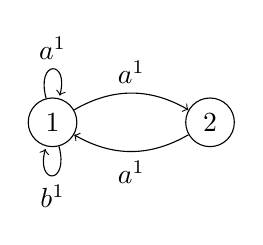
\begin{tikzpicture}
            \graphbox{}{0mm}{0mm}{32mm}{28mm}{-10mm}{-14mm}{
                \node[draw,circle] (1) at (0,0) {1};
                \node[draw,circle] (2) at (2,0) {2};
                \draw[->] (1) edge[loop above] node[midway, above] {$a^{1}$} (1) ;
                \draw[->] (1) edge[loop below] node[midway, below] {$b^{1}$} (1) ;
                \draw[->] (1) edge[bend left] node[midway, above] {$a^{1}$}  (2)  ;
                \draw[->] (2) edge[bend left] node[midway, below] {$a^{1}$} (1)   ;
            }
        \end{tikzpicture}
    %     \caption{}
    %     \label{fig:weighted_type_graph_instance_sfsdsfs}
    % \end{figure}
    \end{center}
    We have \begin{itemize}
        \item $ w_\mathcal{T}(h_{11}^1) = w(e_{13a})^{m_{e_{13a}}(h_{11}^1)} \odot w(e_{31a})^{m_{e_{31a}}(h_{11}^1)} =
     1^1 * 1^1 = 1$
        \item $
        w_\mathcal{T}(h_{11}^2) 
        % = 1^1 * 1^1 
        = 1$
    \end{itemize}
\end{example}   
